\documentclass[10pt]{article}

\usepackage[margin=1in]{geometry}
\usepackage{amsmath,amssymb,amsthm,mathtools}
\usepackage{booktabs,array}
\usepackage{float}
\usepackage{graphicx}
\usepackage{microtype}
\usepackage[hidelinks]{hyperref}
\hypersetup{pdftitle={LSSO: Solved Contextual Operators for Bidirectional Sequence Modeling},
  pdfauthor={Zhaoyang Wang}}

\newtheorem{theorem}{Theorem}[section]
\newtheorem{proposition}[theorem]{Proposition}
\newtheorem{corollary}[theorem]{Corollary}
\newtheorem{definition}[theorem]{Definition}
\newtheorem{remark}[theorem]{Remark}

\newcommand{\R}{\mathbb{R}}
\newcommand{\I}{\mathbf{I}}
\newcommand{\T}{\mathsf{T}}
\newcommand{\norm}[1]{\left\lVert #1 \right\rVert}
\newcommand{\inner}[2]{\left\langle #1, #2 \right\rangle}
\newcommand{\rank}{\operatorname{rank}}
\newcommand{\sym}{\operatorname{sym}}
\newcommand{\diag}{\operatorname{Diag}}
\newcommand{\tril}{\operatorname{tril}}
\newcommand{\triu}{\operatorname{triu}}
\newcommand{\qf}{\operatorname{qf}}

\title{LSSO: Solved Contextual Operators for Bidirectional Sequence Modeling}
\author{Zhaoyang Wang\\\texttt{zhaoy@uir.edu.cn}}
\date{}

\begin{document}
\maketitle

\begin{abstract}
Test-time training constructs an input-specific memory by adapting an internal
model to contextual associations.  For full-context tasks, all positions can
participate in this adaptation, but computing the state through repeated
updates introduces a tradeoff between update budget and execution cost.
We propose LSSO, a bidirectional sequence layer that obtains a shared memory
by solving a compact linear system.  The system is generated from the complete
input and has an exact interpretation as regularized associative-memory error
correction with skew-symmetric coupling.  Its structure guarantees a unique
solution and bounds the forward and adjoint solves.  A shared frame maps the
state back to tokens, yielding a mixer whose spectral norm is strictly below
one and can be computed in compact space for each input.  Forward and backward
costs grow linearly with sequence length at fixed rank.  On eight
GenomicBenchmarks tasks with matched encoders and three seeds, LSSO achieves
the highest mean accuracy on seven tasks and a macro accuracy of $78.53\%$,
compared with $75.57\%$ for the strongest baseline.  On ImageNet-1K, Small and Base models reach $79.43\%$ and
$82.24\%$ validation Top-1 accuracy.  Four Long Range Arena tasks,
diagnostics of trained operators, and CUDA timings further evaluate
sequence accuracy, operator stability, and computational cost.
\end{abstract}

\begin{figure}[t]
\centering
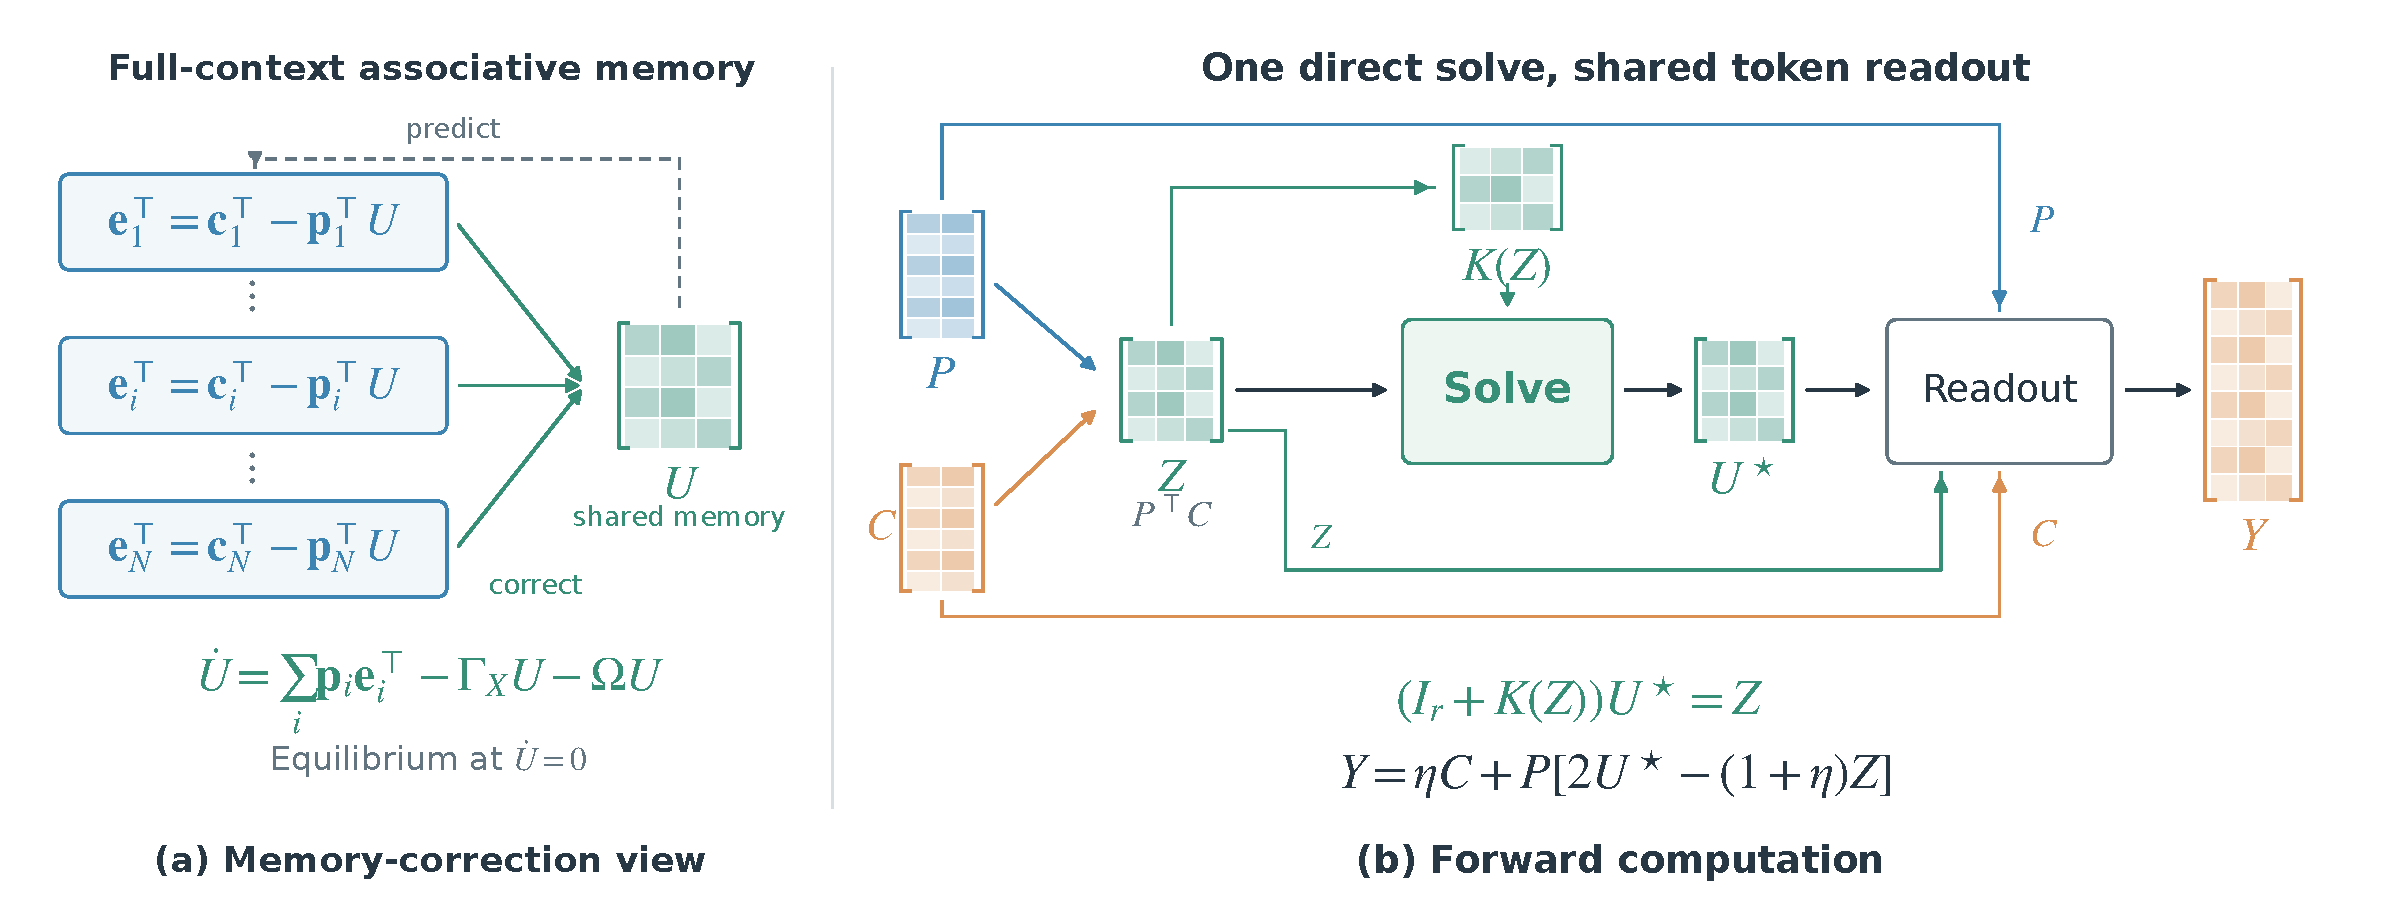
\includegraphics[width=\linewidth]{operator_overview.pdf}
\caption{\textbf{Full-context associative memory in LSSO.}
(a) Each association produces a residual under the same memory $U$.
The weighted residuals, regularization, and skew coupling define the
memory-correction field, with $\Gamma_X=\I_r+LL^\T-P^\T P$.
(b) LSSO evaluates its equilibrium directly: $P$ and $C$ form the statistic
$Z$, which generates $K(Z)$ and supplies the right-hand side of the solve.
The readout combines $U^\star$ with the shared frame, content, and statistic.
Panel (a) is an equivalent dynamics interpretation, not an unrolled computation.
Blue denotes association coordinates, orange denotes content and output,
and green denotes memory quantities.}
\label{fig:overview}
\end{figure}

\section{Introduction}
\label{sec:introduction}

Visual recognition and offline sequence understanding require representations
that combine evidence from across an input.  Pairwise attention provides this
global interaction, but its quadratic arithmetic becomes costly as sequences
grow.  Compact memories offer a different computational route: encode the
context in a bounded state and use that state to inform every output position.
The challenge is to form a memory that captures the associations needed to
interpret the current sample.

Test-time training (TTT) makes this adaptation explicit by treating contextual
associations as training data for an internal model \cite{sun2025ttt}.
The outer network learns how to construct and read that model, while an inner
computation adapts it to the current input.  ViT$^3$ brings this perspective to
visual sequence modeling and studies how the inner learning procedure should
be designed \cite{han2026vit3}.  In its visual experiments, a full-batch inner
update outperforms sequential mini-batch updates; the authors relate this
finding to the causal dependencies and overwriting introduced by sequential
updates.  For tasks with complete input access, this finding supports adapting a shared
memory using all positions together.

Computing this shared state introduces a second problem.  In an error-correcting memory, each association's residual depends
on the current state, and these residuals in turn change that state.  A
full-context update evaluates this feedback across all positions, but a finite
update budget still makes the result depend on the chosen step sizes and
number of steps.  ViT$^3$ illustrates the practical tradeoff: additional
full-batch inner updates can improve accuracy, while reducing throughput and,
in some tested configurations, destabilizing training \cite{han2026vit3}.
We therefore ask whether full-context memory correction can be formulated as
a compact equilibrium problem with a direct solution and a controlled readout.

DeltaNet and MesaNet suggest how to formulate such a problem.  DeltaNet updates memory using the residual
between an association's prediction and target, and efficient chunkwise
algorithms enable parallel training
\cite{schlag2021fastweights,yang2025deltanet}.  MesaNet instead uses conjugate
gradients to solve a contextual regression problem at causal positions
\cite{vonoswald2026mesanet}.  We draw on DeltaNet's residual correction and MesaNet's use of a solve to
construct a shared full-context memory.
The difficulty is to preserve this error-correcting mechanism while making
full-context computation efficient.  LION's Appendix~B.7 gives bidirectional
recurrent and chunkwise DeltaNet formulations, but identifies a bottleneck in
the full-attention expression it considers: a matrix inverse whose cost grows
cubically with sequence length \cite{afzal2025lion}.  Thus, even though this
expression exposes parallel computation, its $O(N^3)$ inversion can dominate
the cost of processing long sequences and negate the intended training
advantage.  LION consequently avoids that full-attention route for DeltaNet
training.  The challenge is therefore to retain global association-error
feedback without solving a system whose dimension grows with the sequence.

We introduce LSSO, which constructs a shared memory equilibrium from the
complete input and evaluates it by one direct solve per sample and head.
A soft association frame $P$ gathers content $C$ into a cross-moment
$Z=P^\T C$, which generates a compact system $K(Z)$.  The memory satisfies
\begin{equation}
    (\I_r+K(Z))U^\star=Z.
\label{eq:intro-state}
\end{equation}
All valid tokens jointly determine this system, but its dimension is the
compact rank $r$, independent of sequence length $N$.  The factorization and
solve cost $O(r^3+r^2d)$ per head, and gathering and reading the context cost
$O(Nr^2+Nrd)$.  This places the expensive solve in memory space while allowing
all positions to participate, giving linear total cost in $N$ at fixed rank.
Strict accretivity makes the equilibrium
unique and bounds the inverse used in the state and adjoint solves.  For fixed
sample-conditioned quantities, the system admits an exact decomposition into
regularized association-error correction and skew-symmetric coupling.  The forward pass computes this equilibrium without
unrolling updates.
A readout through the same association frame then gives each token access to
the shared state.  We choose the readout so that its spectral norm is strictly
below one for each input and is exactly computable from compact matrices.
This bound applies with the generated coefficients fixed; the full network
Jacobian also includes derivatives of those coefficients.  The implementation
uses token--rank products and the small solve, giving linear sequence scaling
at fixed rank without forming a dense token matrix.

The paper makes three contributions:
\begin{enumerate}
    \item We construct a full-context memory layer with a directly solved
    equilibrium and derive its connection to regularized association-error
    correction.
    \item We prove bounds on the state and adjoint solves, characterize the
    compact contraction family, and derive the exact spectral norm of the
    induced token mixer.
    \item We evaluate the layer on ImageNet classification, genomic tasks, and Long
    Range Arena, measure operator margins in trained models, and implement an
    equivalent CUDA forward and backward for timing comparisons.
\end{enumerate}

\section{Related Work}
\label{sec:related-work}

\paragraph{Test-time training and full-context visual adaptation.}
TTT layers treat hidden states as internal models adapted on the current
context \cite{sun2025ttt}.  ViT$^3$ studies the inner objectives, update settings,
and model architectures needed for visual TTT \cite{han2026vit3}.  Its full-batch updates provide a noncausal form of adaptation.  ZipMap likewise
forms a shared scene state from an image collection \cite{jin2026zipmap}.
LSSO defines a different internal system whose equilibrium admits a compact
direct solve.  Work on KV-binding TTT also shows why the quality of an inner
solution must be distinguished from its usefulness for the outer task \cite{liu2026kvbinding}.

\paragraph{Error-correcting memory and solved adaptation.}
Fast-weight interpretations connect linear attention to associative memory;
DeltaNet replaces purely additive storage with prediction-error correction
\cite{schlag2021fastweights,yang2025deltanet}.  Test-time regression provides a
common language for contextual memory objectives
\cite{wang2025testtimeregression}, and Longhorn derives state-space updates
from online learning \cite{liu2024longhorn}.  MesaNet studies contextual
regression solved through conjugate gradients with a chunkwise implementation
\cite{vonoswald2026mesanet}.  LSSO uses these ideas to construct an accretive system from the complete
context.  Section~\ref{sec:memory-correction} derives the corresponding
association-error dynamics, including the role of the skew term.

\paragraph{Bidirectional sequence computation.}
LION gives equivalent full, recurrent, and chunkwise views of bidirectional
linear attention \cite{afzal2025lion}.  Its Appendix~B.7 separates bidirectional
DeltaNet formulations from the matrix-inverse cost of the full-attention
expression it analyzes.  LSSO constructs a different global system with a
solve dimension set by compact rank.  A related architectural route extends
selective SSMs such as Mamba \cite{gu2024mamba,dao2024mamba2}: Hydra uses
quasiseparable matrix mixers to construct a principled bidirectional extension
\cite{hwang2024hydra}.  LSSO's construction starts from a sample-generated
memory equilibrium and its readout.  Matched comparisons with these recent architectures remain future work.

\paragraph{Compact states and global interaction.}
Efficient attention uses projections, kernels, landmarks, or inducing states
to avoid a dense token map
\cite{wang2020linformer,katharopoulos2020linear,choromanski2021performer,
qin2022cosformer,xiong2021nystrom}.  Set Transformer, Luna, ABC, and Perceiver
mediate global interactions through a bounded auxiliary representation
\cite{lee2019settransformer,ma2021luna,peng2022abc,jaegle2021perceiver}.
XCiT uses token-aggregated cross-covariance to generate a shared channel mixer
\cite{ali2021xcit}.  In LSSO, a compact cross-moment generates the system to be solved, and the
same association frame gathers the context and reads out the solution.

\paragraph{Monotone equilibria and contractive parameterization.}
Deep equilibrium models differentiate through implicit states
\cite{bai2019deep}, and monotone operator equilibrium networks impose
structure that makes those states well posed \cite{winston2020mondeq}.
Cayley relations between accretive operators and contractions are classical
\cite{bauschke2017convex}; direct parameterizations also provide complete
charts for static Lipschitz-bounded network weights \cite{wang2023direct}.
LSSO uses these tools for a sample-generated memory equilibrium and its
structured token-space readout.  Its norm analysis fixes the generated coefficients, whereas global Lipschitz
analyses of self-attention must also account for their input dependence \cite{kim2021lipschitz}.

\paragraph{Hardware-efficient execution.}
FlashAttention and hardware-aware SSM algorithms demonstrate the importance of
memory traffic and execution structure alongside arithmetic complexity
\cite{dao2022flashattention,gu2024mamba}.  DeltaNet's chunkwise algorithm also
makes error-correcting memory practical through hardware-efficient training
\cite{yang2025deltanet}.  LSSO lowers its compact equilibrium algebra and
analytic backward to tiled CUDA kernels.  At fixed rank its sequence-dependent
arithmetic is linear, while exact softmax attention retains quadratic
pairwise arithmetic even without materializing its score matrix.
Section~\ref{sec:cuda-implementation} reports complete-mixer measurements;
Appendix~\ref{app:cuda} distinguishes the current implementation from the
historical timing protocol.

\section{LSSO: Full-Context Memory Adaptation}
\label{sec:method}

LSSO first gathers the input into association coordinates, then constructs and
solves a compact memory system, and finally reads the state back to tokens.
The memory-correction interpretation follows from this construction.

We describe one head and omit the batch index.  Let $X\in\R^{N\times D}$ be
the incoming token matrix, $d$ the head width, and $r$ the compact rank.  A
single input projection produces relation and content coordinates
\begin{equation}
    [A,C] = XW_{bc}+b_{bc},
    \qquad A\in\R^{N\times r},\quad C\in\R^{N\times d}.
\label{eq:input-projection}
\end{equation}
Heads are concatenated and passed through an ordinary output projection after
mixing.  The construction below is repeated independently for each head, with
one compact memory state shared by all valid tokens in that head.
The state is recomputed from the current sample; learned outer parameters
remain fixed during each forward evaluation.

\subsection{Overview}
For normalized, position-transformed relation coordinates, LSSO builds a soft
frame $P$ and evaluates
\begin{equation}
 Z=P^\T C,\qquad U^\star=(\I_r+K(Z))^{-1}Z,\qquad
 Y=\eta C+P[2U^\star-(1+\eta)Z].
\label{eq:computation-overview}
\end{equation}
Here $P$ is the association frame, $K$ is generated from $Z$, and $\eta$ is
a learned scalar.  We define each below, starting with the token coordinates
used to construct $P$.

\subsection{Relation features and masking}
\label{sec:masking}

For a boolean validity mask $m\in\{0,1\}^N$, invalid rows of both $A$ and $C$
are set to zero before any compact statistic is formed.  Let
\begin{equation}
    n = \sum_{i=1}^N m_i.
\end{equation}
For a nonempty sequence, relation coordinates are normalized as
$A\leftarrow A/\sqrt{n}$.  An entirely masked sequence is assigned the zero
output by definition.  Masking before normalization makes the result invariant
to appended padding.

The operator consumes relation and content features without an internal
position-dependent transform. Absolute or two-dimensional learned position
embeddings belong to the surrounding encoder.

\subsection{Association frame}
\label{sec:soft-frame}

The QR soft frame maps unconstrained relation coordinates to a strict column
contraction.  Form the reduced QR factorization
\begin{equation}
    \begin{bmatrix}P\\E\end{bmatrix}R_{\mathrm{qr}}
    =
    \begin{bmatrix}A\\\I_r\end{bmatrix},
    \qquad
    \begin{bmatrix}P\\E\end{bmatrix}^{\!\T}
    \begin{bmatrix}P\\E\end{bmatrix}=\I_r,
\label{eq:soft-frame}
\end{equation}
where $P\in\R^{N\times r}$ is the token-space frame.  A common positive
rescaling, which leaves the exact $Q$ factor unchanged, controls the numerical
range.
The identity augmentation means that the factorization is defined even when
$N<r$ or $A$ is rank deficient.

Each row of $P$ supplies an association coordinate, and $C$ supplies its
content target.  A memory $U\in\R^{r\times d}$ predicts those targets as
$PU$.  The frame compresses the content into one shared cross-moment,
\begin{equation}
    Z=P^\T C\in\R^{r\times d}.
\label{eq:cross-moment}
\end{equation}
$Z$ aggregates all valid positions symmetrically in one noncausal pass without
forming the token-level matrix in \eqref{eq:token-mixer}.

\begin{theorem}[Soft-frame spectrum and coverage]
\label{thm:soft-frame}
Let $P$ be the upper block of the $Q$ factor in
\eqref{eq:soft-frame}.  If $\sigma_i(A)$ are the singular values of the
normalized relation matrix, then
\begin{equation}
    \sigma_i(P)=\frac{\sigma_i(A)}
    {\sqrt{1+\sigma_i(A)^2}}.
\label{eq:soft-frame-spectrum}
\end{equation}
Consequently,
\begin{equation}
    P^\T P \prec \I_r,
    \qquad
    \I_N-PP^\T \succ 0,
    \qquad
    1-\norm{P}_2^2=\frac{1}{1+\norm{A}_2^2}.
\label{eq:soft-frame-contract}
\end{equation}
Moreover, at the level of represented frames, the construction covers every
$P\in\R^{N\times r}$ satisfying $P^\T P\prec\I_r$.
\end{theorem}

The lower QR block satisfies $E=R_{\mathrm{qr}}^{-1}$, so
$P^\T P+E^\T E=\I_r$ gives the strict frame margin.
Appendix~\ref{app:proofs} derives the spectrum and proves coverage of the
represented frame family.

The identity augmentation supplies the strict complement $\I_N-PP^\T$, which
allows the compact contraction to extend to every token direction.  If $A_0$ denotes
the masked relation matrix before division by $\sqrt n$, the final term in
\eqref{eq:soft-frame-contract} becomes
$1/(1+\norm{A_0}_2^2/n)$.  Thus bounded per-token relation energy prevents the
frame margin from deteriorating merely because the sequence is longer.


\subsection{Memory system}
\label{sec:accretive-core}

In the default \textsc{Dynamic} mode, $Z$ generates compact raw coordinates
\begin{equation}
    \Theta = \Theta_0 + \frac{ZW_{\mathrm{drive}}}{\sqrt{n}},
\label{eq:dynamic-coordinates}
\end{equation}
where $\Theta_0\in\R^{r\times r}$ and
$W_{\mathrm{drive}}\in\R^{d\times r}$ are learned per-head parameters.  The
\textsc{Static} ablation uses $\Theta=\Theta_0$, while \textsc{Zero} fixes the
compact contraction to zero.

\begin{definition}[Strict accretivity]
\label{def:accretive}
A real square matrix $K$ is strictly accretive when
\begin{equation}
    \sym(K) \coloneqq \frac{K+K^\T}{2}\succ0.
\end{equation}
\end{definition}

For \textsc{Dynamic} and \textsc{Static}, define
\begin{align}
    L(\Theta) & = \tril(\Theta,-1)+
        \diag\!\left(\operatorname{softplus}
        \bigl(\operatorname{diag}(\Theta)+c_1\bigr)\right), \\
    \Omega(\Theta) & = \triu(\Theta,1)-\triu(\Theta,1)^\T, \\
    K(\Theta) & = L(\Theta)L(\Theta)^\T+\Omega(\Theta),
\label{eq:accretive-parameterization}
\end{align}
where $c_1=\operatorname{softplus}^{-1}(1)$.  Thus $L$ is lower triangular
with positive diagonal, while $\Omega$ is skew-symmetric.  The compact
equilibrium and the pre-output token coordinates are
\begin{align}
    U^\star &=(\I_r+K)^{-1}Z, \\
    Y &= \eta C+P\left[2U^\star-(1+\eta)Z\right],
    \qquad \eta=\tanh(\eta_{\mathrm{raw}})\in(-1,1).
\label{eq:equilibrium-readout}
\end{align}
The complement is learned independently for each head and is initialized to
$0.9$.  In \textsc{Zero}, $M=0$, which gives
\begin{equation}
    Y=\eta(C-PZ).
\label{eq:zero-core}
\end{equation}
At $\Theta=0$, $L=\I_r$, $\Omega=0$, $K=\I_r$, and the compact contraction is
$M=0$.  Both nonzero-core modes start at that point; \textsc{Dynamic} also
starts with $W_{\mathrm{drive}}=0$.

\subsection{Association-error correction}
\label{sec:memory-correction}

For \textsc{Dynamic} and \textsc{Static}, the constructed system has a precise
error-correction interpretation.  Fix the current sample's $P$, $C$, $L$, and
$\Omega$, and define the derived regularizer
\begin{equation}
    \Gamma_X=\I_r+LL^\T-P^\T P\succ0.
\label{eq:memory-regularizer}
\end{equation}
Positive definiteness follows from Theorem~\ref{thm:soft-frame} and
$LL^\T\succ0$.  The coefficients are fixed during the solve.  In particular, $\Gamma_X$ is
derived from the frame and system parameters rather than learned separately.

\begin{proposition}[Associative-memory correction identity]
\label{prop:memory-correction}
For the fixed contextual quantities above, let
\begin{equation}
    \mathcal J_X(U)=\frac12\norm{PU-C}_F^2
        +\frac12\operatorname{tr}(U^\T\Gamma_XU).
\label{eq:association-objective}
\end{equation}
Then the memory-correction field satisfies
\begin{align}
    \dot U
    &=\underbrace{P^\T(C-PU)}_{\text{association-error feedback}}
       -\Gamma_XU-\Omega U \\
    &=-\nabla_U\mathcal J_X(U)-\Omega U
      =Z-(\I_r+K)U.
\label{eq:memory-correction-flow}
\end{align}
Its unique equilibrium is the state $U^\star$ used by LSSO.
\end{proposition}

\begin{proof}
Since $\Gamma_X$ is symmetric,
$\nabla_U\mathcal J_X(U)=(P^\T P+\Gamma_X)U-P^\T C
=(\I_r+LL^\T)U-Z$.  Adding the skew term gives
$Z-(\I_r+LL^\T+\Omega)U=Z-(\I_r+K)U$.
The symmetric part of $\I_r+K$ is positive definite, so its zero is unique.
\end{proof}

Writing row $i$ of $P$ as $\mathbf p_i^\T$ and row $i$ of $C$ as $\mathbf c_i^\T$ makes the
feedback explicit:
\begin{equation}
    P^\T(C-PU)=\sum_{i:m_i=1}\mathbf p_i(\mathbf c_i^\T-\mathbf p_i^\T U).
\label{eq:association-feedback}
\end{equation}
Every valid association contributes its prediction error to the same memory.
When $\Omega=0$, this is gradient flow on the strictly convex regularized
association objective.  With nonzero $\Omega$, it is a monotone correction
system with skew coupling; $U^\star$ need not minimize
$\mathcal J_X$ itself.  Appendix~\ref{sec:solved-inner-process} proves global
convergence to $U^\star$ for the continuous process, while
Section~\ref{sec:theory} bounds the solve and its implicit adjoint.

The forward pass obtains this equilibrium by solving the $r\times r$ system.
Backpropagation differentiates through the solve and through the generation of
its coefficients.  The identity explains the memory corrected by LSSO; it
does not require executing the continuous dynamics.

\subsection{Token readout}

Define the reflected resolvent
\begin{equation}
    M = 2(\I_r+K)^{-1}-\I_r
      = (\I_r-K)(\I_r+K)^{-1}.
\label{eq:cayley}
\end{equation}
Substituting $Z=P^\T C$ into \eqref{eq:equilibrium-readout} gives the exact
token-mixing form
\begin{equation}
    Y=TC,\qquad
    T=\eta\I_N+P(M-\eta\I_r)P^\T.
\label{eq:token-mixer}
\end{equation}

\subsection{Linear sequence complexity}
\label{sec:linear-complexity}

For one head, frame formation costs $O(Nr^2)$, the two frame--content
contractions cost $O(Nrd)$, and construction and solution of the compact
problem cost $O(r^2d+r^3)$.  The forward arithmetic and activation/workspace
storage are therefore
\begin{align}
    \mathcal C_{\mathrm{LSSO}}
        &=O\!\left(Nr^2+Nrd+r^2d+r^3\right), \\
    \mathcal M_{\mathrm{LSSO}}
        &=O\!\left(N(r+d)+r^2+rd\right).
\label{eq:lsso-complexity}
\end{align}
The analytic backward reuses compact factors and performs the same classes of
token--rank contractions, so its arithmetic and saved-state dependence on $N$
is also linear.  Multiplying the head-local terms by the number of heads does
not change the sequence-length degree.

Unlike exact MHA, whose $O(N^2d)$ mixing cost persists under FlashAttention
\cite{dao2022flashattention}, LSSO has $O(Nr(r+d))$ token-dependent work and no
$N\times N$ intermediate.  Both retain $O(ND^2)$ feature projections.

\section{Properties of the Memory and Readout}
\label{sec:theory}

We analyze the adaptation state and its induced readout for one realized
head in exact arithmetic.  We first bound the solve and its derivatives, then characterize the compact
operator family and the spectral norm of the token readout.  Complete proofs
are given in Appendix~\ref{app:proofs}, and mixed-precision execution is
described in Section~\ref{sec:cuda-implementation}.

\subsection{Well-posed adaptation and implicit differentiation}

\begin{theorem}[Stable solved state and implicit adjoint]
\label{thm:stable-solve}
Define the per-sample monotonicity margin
\begin{equation}
    \mu=1+\sigma_{\min}(L)^2>1,
    \qquad A_K=\I_r+K.
\label{eq:monotonicity-margin}
\end{equation}
Then $U^\star=A_K^{-1}Z$ exists uniquely, and
\begin{equation}
    \sigma_{\min}(A_K)\geq\mu,
    \quad
    \norm{U^\star}_F\leq\mu^{-1}\norm{Z}_F,
    \quad
    \norm{A_K^{-\T}G}_F\leq\mu^{-1}\norm{G}_F.
\label{eq:solve-adjoint-bound}
\end{equation}
For a second generated problem $A_K'=\I_r+K'$ with margin $\mu'$ and solution
$U^{\star'}=A_K'^{-1}Z'$, the finite contextual perturbation obeys
\begin{equation}
    \norm{U^\star-U^{\star'}}_F
    \leq \mu^{-1}\norm{Z-Z'}_F
       +(\mu\mu')^{-1}\norm{K-K'}_2\norm{Z'}_F.
\label{eq:finite-solve-sensitivity}
\end{equation}
Consequently, an infinitesimal perturbation obeys
\begin{equation}
    \norm{dU^\star}_F
    \leq \mu^{-1}\norm{dZ}_F
       +\mu^{-2}\norm{dK}_2\norm{Z}_F.
\label{eq:solve-sensitivity}
\end{equation}
\end{theorem}

The same computable margin controls the forward state, the transposed solve
used by implicit differentiation, and sensitivity to the generated compact
problem.  The realized-gain certificate below separately measures the
contraction margin, which also depends on the skew coordinates.

\subsection{Context dependence and expressivity}

\begin{proposition}[Length-normalized contextual drive]
\label{prop:length-normalized-drive}
For the dynamic core,
\begin{equation}
    \norm{Z}_F\leq\norm{P}_2\norm{C}_F,
    \qquad
    \norm{\Theta-\Theta_0}_F
    \leq \frac{\norm{C}_F}{\sqrt n}\norm{W_{\mathrm{drive}}}_2.
\label{eq:length-normalized-drive}
\end{equation}
The first inequality is strict relative to $\norm{C}_F$ whenever $C\neq0$.
Accordingly, if $\norm{C}_F^2/n\leq c^2$, the magnitude of the contextual
drive is at most $c\norm{W_{\mathrm{drive}}}_2$, independently of sequence
length.
\end{proposition}

\paragraph{A complete compact contraction chart.}



The Cayley connection between accretive coordinates and contractions is
classical in monotone operator theory \cite{bauschke2017convex}, and direct
Cayley charts have parameterized static Lipschitz-bounded network weights
\cite{wang2023direct}.  We use this relation to characterize the compact maps represented by LSSO.

\begin{theorem}[Accretive Cayley parameterization]
\label{thm:accretive-cayley}
The map in \eqref{eq:accretive-parameterization} ranges over all real
strictly accretive $r\times r$ matrices.  For every such $K$, the reflected
resolvent $M$ in \eqref{eq:cayley} is a strict spectral-norm contraction and
obeys
\begin{equation}
    \I_r-M^\T M
    =4(\I_r+K)^{-\T}L L^\T(\I_r+K)^{-1}\succ0.
\label{eq:cayley-defect}
\end{equation}
Conversely, the map $K\mapsto M$ is a bijection from real strictly accretive
matrices to the open real matrix ball $\{M:\norm{M}_2<1\}$, with inverse
\begin{equation}
    K=(\I_r-M)(\I_r+M)^{-1}.
\label{eq:inverse-cayley}
\end{equation}
\end{theorem}

\begin{proof}[Proof sketch]
The construction has
$\sym(K)=LL^\T\succ0$, because $L$ has positive diagonal.  Conversely, for
any strictly accretive $K$, the Cholesky factor of $\sym(K)$ and the skew
remainder $K-\sym(K)$ recover $L$ and $\Omega$, proving completeness.

Let $Q=\I_r+K$.  Strict accretivity implies that $Q$ is nonsingular.  Using
$M=(\I_r-K)Q^{-1}$ gives
\begin{align}
    \I_r-M^\T M
    &=Q^{-\T}\left[Q^\T Q-(\I_r-K)^\T(\I_r-K)\right]Q^{-1}\\
    &=4Q^{-\T}\sym(K)Q^{-1},
\end{align}
which is \eqref{eq:cayley-defect}.  It is positive definite, so
$\norm{M}_2<1$.
The inverse formula maps every strict contraction back to a strictly
accretive matrix.
\end{proof}

Because $\Omega$ is unrestricted, $K$ and $M$ may be nonsymmetric and
nonnormal.  The chart retains every strict contraction in rank space, and at
token level,
$T-T^\T=P(M-M^\T)P^\T$, so this nonsymmetric structure survives the lift.

\subsection{Exact gain of the global readout}

The soft frame identifies the token subspace where contextual mixing acts.
Figure~\ref{fig:geometry} separates this compact action from the scalar
complement.  Because $P$ is generally not orthonormal, the restricted token
block $B$ below differs from the compact Cayley core $M$.

\begin{figure}[t]
\centering
\includegraphics[width=\linewidth]{operator_geometry.pdf}
\caption{\textbf{From token subspaces to an exact gain.}
(a) An illustrative nonsymmetric contraction in the frame subspace and scalar
multiplication on its orthogonal complement; the scalar sketch uses positive
$\eta$.  (b) In an orthonormal token basis, the realized mixer separates into
$B$ and $\eta I$.  (c) For $0<k<N$, its norm is the larger of the two block norms.
Theorem~\ref{thm:token-contraction} covers either sign of $\eta$ and the empty
and full-rank cases.  The ellipse and matrix glyphs are schematic, not trained
operator measurements.}
\label{fig:geometry}
\end{figure}


\begin{theorem}[Exact realized-gain certificate]
\label{thm:token-contraction}
Fix a sample and head, and let $P$, $M$, and $\eta$ be constructed as above.
Write the positive eigenspace of $P^\T P$ as
\begin{equation}
    P^\T P=V_kS^2V_k^\T,
    \qquad k=\rank(P),
\end{equation}
where $S\in\R^{k\times k}$ is positive diagonal, and define
\begin{equation}
    B=\eta\I_k+SV_k^\T(M-\eta\I_r)V_kS.
\label{eq:compact-certificate-block}
\end{equation}
Then the singular values of $T$ are exactly those of $B$, together with
$N-k$ copies of $|\eta|$.  Equivalently,
\begin{equation}
 q(X)\coloneqq\norm{T}_2=
 \begin{cases}
   |\eta|, & k=0,\\
   \sigma_{\max}(B), & k=N,\\
   \max\{\sigma_{\max}(B),|\eta|\}, & 0<k<N,
 \end{cases}
 \qquad q(X)<1.
\label{eq:exact-token-gain}
\end{equation}
Moreover, $\rank(T-\eta\I_N)\leq r$ and
$Tv=\eta v$ for every $v\in\ker(P^\T)$.
\end{theorem}

\begin{proof}[Proof sketch]
Let $Q=PV_kS^{-1}$.  Then $Q^\T Q=\I_k$, and substitution gives
$T=QBQ^\T+\eta(\I_N-QQ^\T)$, so an orthogonal basis containing $Q$ yields the
stated singular spectrum.  With $\Delta=(\I_N-PP^\T)^{1/2}$ and
$F=[P\;\Delta]$,
\begin{equation}
    T=F\diag(M,\eta\I_N)F^\T,
\label{eq:defect-completion}
\end{equation}
and $FF^\T=\I_N$; hence $\norm{T}_2<1$.  Finally,
$T-\eta\I_N=P(M-\eta\I_r)P^\T$, which gives both the rank bound and
$Tv=\eta v$ on $\ker(P^\T)$.
\end{proof}

The exact certificate requires only an
$r\times r$ Gram eigendecomposition and a singular-value calculation of size
at most $r\times r$; no $N\times N$ kernel is needed.  Because the forward uses the
input-dependent $T(X)$ itself, Equation~\eqref{eq:exact-token-gain} gives the
pointwise energy statement
\begin{equation}
    \norm{T(X)C(X)}_F\leq q(X)\norm{C(X)}_F<\norm{C(X)}_F
\label{eq:pointwise-energy}
\end{equation}
whenever $C(X)\neq0$.  The guarantee is pointwise in the input-conditioned
operator.  It does not bound the Jacobian of $X\mapsto T(X)C(X)$,
which also contains $(dT)C$.  Along any fixed realized sequence of mixer maps, the gains compose:
$\norm{T_L\cdots T_1}_2\leq\prod_{\ell=1}^L q_\ell$.

\begin{remark}[Why the scalar complement is part of the model]
\label{rem:complement}
Without the complement, a conventional form $\I_N+PAP^\T$ fixes the entire
$\ker(P^\T)$ subspace to gain one.  Equation~\eqref{eq:defect-completion}
instead assigns that unmodeled subspace the learned per-head scalar $\eta$,
while retaining the same rank-$r$ correction and the strict contraction
certificate.  Thus $T$ is a rank-$r$ correction to an isotropic complement.
\end{remark}

Appendix~\ref{app:proofs} proves padding isolation and noncausal permutation
equivariance.

\section{Experiments}
\label{sec:sequence-experiments}

We evaluate LSSO in image classifiers and bidirectional sequence encoders.
ImageNet training follows the DeiT III protocol.
The accuracy and timing tables retain their original source revisions. Those
runs included a position-dependent relation-feature transform that is absent
from the current operator. They therefore describe the archived models, not
new measurements of the current implementation.
The archived genomic and LRA experiments use the \textsc{Dynamic} core,
rank $32$, FP16 automatic mixed precision, and the CUDA implementation.  For these sequence experiments, checkpoints are
selected only by validation accuracy, with validation loss breaking an exact
tie; the held-out test split is evaluated once after selection.  Reported
uncertainties are sample standard deviations over seeds $0$, $1$, and $2$.
Across the genomic and LRA configurations, LSSO requires
$1.3\%$--$32.0\%$ of exact MHA's sequence-dependent mixer-core MACs
(Appendix~\ref{app:mixer-macs}).

\subsection{ImageNet classification}
\label{sec:vision}

\paragraph{Experimental settings.}
We evaluate image classification on ImageNet-1K, which contains 1.28M training
images and 50K validation images from 1,000 classes
\cite{russakovsky2015imagenet}.  We replace the attention layers in DeiT III
with LSSO and follow the DeiT III training protocol \cite{touvron2022deit3}.
Both Small and Base use 12 blocks, $16\times16$ patches, and a class-token
readout.  Their widths, head counts, and compact ranks are $(384,6,32)$ and
$(768,12,48)$, respectively.  All LSSO layers use the \textsc{Dynamic} core.

We train for 800 epochs with fused LAMB and a total batch size of 2048, using
3-Augment, Mixup, CutMix, and binary cross-entropy.  Small is trained at
$224\times224$; Base is trained at $192\times192$ and then fine-tuned for
20 epochs at $224\times224$ with AdamW and a batch size of 512.
We report validation Top-1 accuracy at $224\times224$.  Checkpoint selection
and full training settings are provided in Appendix~\ref{app:imagenet-protocol}.

\begin{table}[H]
\centering
\small
\setlength{\tabcolsep}{5pt}
\caption{ImageNet-1K classification at $224\times224$.  All models use
ImageNet-1K training data only.  Baseline results are quoted from the cited
papers or official releases under their respective training protocols;
LSSO follows DeiT III.  Training schedules, augmentation, and other settings
are not unified across methods.}
\label{tab:imagenet-comparison}
\begin{tabular}{llrr}
\toprule
Model & Mixing mechanism & Params (M) & Top-1 (\%) \\
\midrule
\multicolumn{4}{l}{\emph{Established classification baselines}} \\
DeiT-S \cite{touvron2021deit} & Self-attention & 22 & 79.8 \\
DeiT-B \cite{touvron2021deit} & Self-attention & 86 & 81.8 \\
DeiT III-S \cite{touvron2022deit3} & Self-attention & 22.0 & 81.4 \\
DeiT III-B \cite{touvron2022deit3} & Self-attention & 86.6 & 83.8 \\
ConvNeXt-T \cite{liu2022convnext} & Convolution & 28 & 82.1 \\
ConvNeXt-B \cite{liu2022convnext} & Convolution & 89 & 83.8 \\
\midrule
\multicolumn{4}{l}{\emph{Bidirectional sequence mixers and visual TTT}} \\
Vim-S \cite{zhu2024vim} & Bidirectional SSM & 26 & 80.3 \\
Vim-B \cite{zhu2024vim} & Bidirectional SSM & 98 & 81.9 \\
Vim-S$^\dagger$ \cite{zhu2024vim} & Bidirectional SSM & 26 & 81.4 \\
Vim-B$^\dagger$ \cite{zhu2024vim} & Bidirectional SSM & 98 & 83.2 \\
Hydra-ViT-B \cite{hwang2024hydra} & Bidirectional SSM & 91 & 81.6 \\
LION-D$^\natural$ (Small) \cite{afzal2025lion} & Bidirectional linear attention & 22 & 79.9 \\
LION-D$^\natural$ (Base) \cite{afzal2025lion} & Bidirectional linear attention & 86 & 80.2 \\
ViT$^3$-S \cite{han2026vit3} & Test-time training & 24 & 81.6 \\
ViT$^3$-B \cite{han2026vit3} & Test-time training & 90 & 82.6 \\
\midrule
\multicolumn{4}{l}{\emph{Our models}} \\
LSSO-S & Associative memory & 19.62 & 79.43 \\
LSSO-B & Associative memory & 78.50 & 82.24 \\
\bottomrule
\end{tabular}
\par\smallskip
\begin{minipage}{0.96\linewidth}
\footnotesize
$\dagger$: Vim fine-tuned for 30 additional epochs at $224\times224$ with
patch size 16 and extraction stride 8.  $\natural$: LION with multiple scans.
\end{minipage}
\end{table}

\paragraph{Results.}
Table~\ref{tab:imagenet-comparison} compares LSSO with established classifiers
and related bidirectional sequence models.  LSSO-S achieves $79.43\%$ Top-1
with $19.62$M parameters, and LSSO-B achieves $82.24\%$ with $78.50$M.
LSSO-B is $0.44$ points above the quoted DeiT-B result and $0.36$ points below
ViT$^3$-B, while DeiT III-B reaches $83.8\%$.  These comparisons place LSSO
among existing visual backbones, but differences in training protocols
prevent attributing the accuracy differences to the mixer alone.

\subsection{Genomic classification}

GenomicBenchmarks collects binary DNA sequence-classification tasks with
official train and test partitions \cite{gresova2023genomicbenchmarks}.  We
derive a deterministic stratified validation set only from each training
partition.  All mixers use the same $D=128$, four-layer, four-head encoder,
learned absolute position embeddings, MLP ratio $4$, mean readout, optimizer,
data order, and $40$-epoch budget; only the token mixer changes.  Alongside MHA,
we test bidirectional ELU${}+1$ Linear Transformer
\cite{katharopoulos2020linear}, FAVOR$+$ Performer with fixed orthogonal
random features \cite{choromanski2021performer}, and the official bidirectional
ReLU/cosine cosFormer formulation \cite{qin2022cosformer}.  Numerically
sensitive attention cores run in FP32 under automatic mixed precision.  The
effective batch is $128$, using two-step accumulation for Mouse Enhancers
Ensembl.  The three linear baselines match MHA's parameter count; LSSO is
$4.1\%$ smaller on the 200-position tasks.

\begin{table}[H]
\centering
\footnotesize
\setlength{\tabcolsep}{3.2pt}
\caption{GenomicBenchmarks held-out test accuracy (\%), mean $\pm$ sample
standard deviation over three seeds under the matched encoder and training
protocol.  Bold marks the highest mean in each row.}
\label{tab:genomic-results}
\begin{tabular}{lrrrrr}
\toprule
Task & MHA & Linear & Performer & cosFormer & LSSO \\
\midrule
Coding vs. intergenomic  & $80.34\pm1.99$ & $78.11\pm0.10$ & $78.17\pm0.01$ & $79.12\pm0.05$ & $\boldsymbol{83.23\pm2.46}$ \\
Human or worm            & $65.87\pm0.35$ & $65.68\pm0.22$ & $65.76\pm0.08$ & $66.07\pm0.20$ & $\boldsymbol{81.57\pm1.18}$ \\
Mouse enhancers Ensembl  & $71.07\pm1.65$ & $\boldsymbol{71.63\pm0.48}$ & $71.35\pm0.48$ & $71.35\pm0.48$ & $70.25\pm0.83$ \\
Human enhancers Cohn     & $66.83\pm0.17$ & $66.89\pm0.07$ & $67.16\pm0.08$ & $67.06\pm0.23$ & $\boldsymbol{67.24\pm0.26}$ \\
Human enhancers Ensembl  & $76.37\pm0.20$ & $75.16\pm0.57$ & $74.32\pm0.23$ & $77.34\pm1.53$ & $\boldsymbol{78.91\pm0.05}$ \\
Human regulatory         & $92.14\pm0.05$ & $91.79\pm0.15$ & $90.10\pm0.34$ & $92.65\pm0.14$ & $\boldsymbol{93.10\pm0.02}$ \\
Human non-TATA promoters & $84.71\pm0.15$ & $80.44\pm1.84$ & $82.51\pm1.07$ & $84.42\pm0.48$ & $\boldsymbol{85.41\pm0.17}$ \\
Human OCR Ensembl        & $65.61\pm0.54$ & $65.12\pm0.26$ & $65.36\pm0.27$ & $66.56\pm0.07$ & $\boldsymbol{68.55\pm0.31}$ \\
\midrule
Unweighted task macro    & $75.37$ & $74.35$ & $74.34$ & $75.57$ & $\mathbf{78.53}$ \\
\bottomrule
\end{tabular}
\end{table}

Table~\ref{tab:genomic-results} shows that LSSO has the highest mean on
seven of eight tasks.  Its $78.53$ macro average exceeds cosFormer, the strongest alternative
at $75.57$, by $2.96$ points and MHA's $75.37$ by $3.16$ points.  The largest improvement is on Human or Worm, while Linear Transformer leads
on Mouse Enhancers Ensembl.  The small mean differences on tasks such as
Human Enhancers Cohn should be read alongside the three-seed variability.
The macro average weights tasks equally after averaging seeds within each task.

\subsection{Long Range Arena}

Long Range Arena (LRA) tests structured reasoning and long-context
classification \cite{tay2021lra}.  Following established reporting practice
\cite{gu2022s4}, Table~\ref{tab:lra-results} quotes results from the original
benchmark and subsequent work and groups models by their primary mixing
mechanism.  General-purpose global mixers and efficient-attention
approximations form the first block; structured recurrence and state-space
models form the second.  These published results use different training protocols; locality and
positional design also affect performance \cite{mirallesgonzalez2025locality}.

We evaluate LSSO on four LRA tasks using six-layer encoders, with $D=128$ for
ListOps and Retrieval and $D=256$ for Text and Pathfinder-32.  ListOps, Text,
and Retrieval use learned one-dimensional absolute position embeddings with
mean pooling; Pathfinder-32 uses factorized row/column embeddings and
mean--maximum pooling.  Their maximum sequence lengths are $2048$, $4096$,
$4000$, and $1024$, respectively.

\begin{table}[H]
\centering
\footnotesize
\setlength{\tabcolsep}{2.5pt}
\caption{LRA test accuracy (\%) quoted from the cited sources under their
reported protocols.  The four-task average is unweighted over the displayed
tasks.  For LSSO, task scores and the per-seed four-task average are reported as
mean $\pm$ sample standard deviation across three seeds.  Bold marks the
highest reported mean within each mechanism block.}
\label{tab:lra-results}
\begin{tabular}{lrrrrr}
\toprule
Model and source & ListOps & Text & Retrieval & Pathfinder & 4-task Avg. \\
\midrule
\multicolumn{6}{l}{\emph{General-purpose global mixers and efficient-attention approximations}} \\
Transformer \cite{tay2021lra} & $36.37$ & $64.27$ & $57.46$ & $71.40$ & $57.38$ \\
Linear Transformer \cite{tay2021lra} & $16.13$ & $\mathbf{65.90}$ & $53.09$ & $75.30$ & $52.61$ \\
Performer \cite{tay2021lra} & $18.01$ & $65.40$ & $53.82$ & $77.05$ & $53.57$ \\
Linformer \cite{tay2021lra} & $35.70$ & $53.94$ & $52.27$ & $76.34$ & $54.56$ \\
Reformer \cite{tay2021lra} & $37.27$ & $56.10$ & $53.40$ & $68.50$ & $53.82$ \\
Luna-256 \cite{ma2021luna}
    & $\mathbf{37.98}$ & $65.78$ & $79.56$ & $78.55$ & $65.47$ \\
FNet \cite{leethorp2022fnet} & $35.33$ & $65.11$ & $59.61$ & $77.80$ & $59.46$ \\
Nystr\"omformer \cite{xiong2021nystrom}
    & $37.15$ & $65.52$ & $79.56$ & $70.94$ & $63.29$ \\
\textbf{LSSO}, three seeds
    & $37.60\pm0.65$ & $65.19\pm0.46$ & $\boldsymbol{82.88\pm0.08}$
    & $\boldsymbol{78.79\pm0.34}$ & $\boldsymbol{66.11\pm0.24}$ \\
\midrule
\multicolumn{6}{l}{\emph{Models centered on structured recurrence or state-space dynamics}} \\
S4, original \cite{gu2022s4}  & $58.35$ & $76.02$ & $87.09$ & $86.05$ & $76.88$ \\
S4-LegS, updated \cite{gu2022hippo}
    & $59.60\pm0.07$ & $86.82\pm0.13$ & $90.90\pm0.15$ & $94.20\pm0.25$ & $82.88$ \\
Mega \cite{ma2023mega} & $\mathbf{63.14}$ & $\mathbf{90.43}$
    & $\mathbf{91.25}$ & $\mathbf{96.01}$ & $\mathbf{85.21}$ \\
\bottomrule
\end{tabular}
\end{table}

Within the global-mixer block, LSSO gives the highest Retrieval, Pathfinder,
and four-task average; it is within $0.38$ points of the highest ListOps result
and $0.71$ points of the highest Text result.  S4 and Mega obtain higher scores across all four tasks.  The table places
LSSO among published results; the matched genomic experiment provides the
controlled comparison of mixers.

\subsection{Operator margins in trained models}
\label{sec:certificate-evidence}

We next test whether trained operators remain comfortably within the bounds
of Section~\ref{sec:theory}.  Across three
six-layer LRA Text checkpoints and matched held-out token-stream probes from
$1$K to $8$K, all $9{,}216$ head-level observations are finite and satisfy
their certified conditions (Table~\ref{tab:certificate-audit}).  The worst
realized gain is $0.9087$, leaving at least $0.0913$ contraction slack, and the
minimum monotonicity margin is $1.1667$.  Solved states use at most $93.3\%$ of
their certified bound, while deterministic adjoint probes use at most $88.1\%$.
Appendix~\ref{app:certificate-protocol} reports the per-layer distributions
and stress-test protocol.

\begin{table}[H]
\centering
\small
\setlength{\tabcolsep}{7pt}
\caption{Worst observation in the trained-model certificate audit.  Bound
usage is the measured ratio normalized by its certified upper bound $1/\mu$.}
\label{tab:certificate-audit}
\begin{tabular}{lcc}
\toprule
Quantity & Certified condition & Worst observed \\
\midrule
Realized gain & $q(X)<1$ & $\max q=0.9087$ \\
Contraction slack & $1-q(X)>0$ & $\min(1-q)=0.0913$ \\
Monotonicity margin & $\mu>1$ & $\min\mu=1.1667$ \\
Solved-state bound usage & $\mu\norm{U^\star}_F/\norm{Z}_F\leq1$ & $0.9329$ \\
Adjoint-probe bound usage & $\mu\norm{A_K^{-\T}G}_F/\norm{G}_F\leq1$ & $0.8814$ \\
\bottomrule
\end{tabular}
\end{table}


The gain in these probes is dominated by the scalar complement $|\eta|$
(Appendix~\ref{app:certificate-protocol}).  The nearly constant worst-case gain therefore reflects the learned complement;
it does not measure how strongly the dynamic core contributes to predictions.
The $8$K probes are operator stress tests on assembled token streams, not an
$8$K classification or length-generalization result.

\subsection{Runtime}
\label{sec:cuda-implementation}

The \textsc{Dynamic}, \textsc{Static}, and \textsc{Zero} cores have a native,
algebraically equivalent CUDA path for inference and first-order training.  It
avoids both the $N\times N$ token matrix and the compact Cayley matrix; compact
factorization and tiled solves evaluate the equilibrium directly, while the
analytic backward reuses saved factors.  Mixed-precision outputs and gradients
are validated against the FP64 reference.  Appendix~\ref{app:cuda} gives the
execution schedule, workspace, VJP, numerical envelope, and build coverage.

These timings use the implementation and software versions recorded in
Appendix~\ref{app:cuda}, rather than the subsequently revised backend.
Table~\ref{tab:cuda-wall-clock} measures the complete mixer boundary, including
input and output projections.  At $N=4096$, native LSSO reaches $1.79\times$
the Flash-SDPA MHA forward throughput and $2.30\times$ its training throughput.
Across $N=1024$--$4096$, forward--backward latency grows by $3.88\times$ for
LSSO and $7.92\times$ for MHA.  At $N=1024$, LSSO is slower in inference ($2.539$ versus $2.131$ ms),
so the throughput advantage depends on sequence length.  The timings cover
the mixer, including projections, rather than the complete encoder.

\begin{table}[H]
\centering
\footnotesize
\setlength{\tabcolsep}{4pt}
\caption{Synchronized milliseconds per batch on an RTX 5070 Ti (lower is
better), with $B=64,D=256,H=8$, FP16 AMP, and $r=32$ for LSSO
(historical contract 6).  Ratios above
one favor native LSSO; forward--backward includes loss and gradient reset.
Bold marks the lowest latency in each row.}
\label{tab:cuda-wall-clock}
\begin{tabular}{lrrrrr}
\toprule
$N$ & PyTorch ref. & Native & MHA & Ref./native & MHA/native \\
\midrule
\multicolumn{6}{l}{\emph{Inference forward}} \\
1024 & 110.216 & 2.539  & $\mathbf{2.131}$  & $43.41\times$ & $0.84\times$ \\
2048 & 133.940 & $\mathbf{5.577}$  & 5.888  & $24.02\times$ & $1.06\times$ \\
4096 & 169.549 & $\mathbf{10.135}$ & 18.173 & $16.73\times$ & $1.79\times$ \\
\midrule
\multicolumn{6}{l}{\emph{Forward--backward with gradient reset}} \\
1024 & 118.858 & $\mathbf{7.512}$  & 8.487  & $15.82\times$ & $1.13\times$ \\
2048 & 153.955 & $\mathbf{15.260}$ & 22.940 & $10.09\times$ & $1.50\times$ \\
4096 & 211.268 & $\mathbf{29.160}$ & 67.195 & $7.25\times$  & $2.30\times$ \\
\bottomrule
\end{tabular}
\end{table}

\section{Limitations}
\label{sec:limitations}

LSSO compresses the associations in a sequence into a memory of fixed rank.
For each sample, the frame selects at most $r$ token directions for nontrivial
mixing; the orthogonal complement receives the same scalar action $\eta$.
Although the frame adapts to the input, a fixed rank may limit the number of
independent relations that one head can represent in a complex context.
Increasing $r$ expands this capacity, but raises the frame cost as $O(Nr^2)$
and the factorization cost as $O(r^3)$.  Linear scaling with sequence length
therefore comes with a capacity--computation tradeoff.

The direct solve also introduces overhead that is not amortized on every
workload.  In our measurements, LSSO has lower inference throughput than
Flash-SDPA attention at $N=1024$, with an advantage emerging at longer lengths.
The crossover depends on model dimensions, precision, and hardware, so linear
asymptotic complexity alone does not imply lower latency.  The current
architecture uses a single global memory per head; combining it with explicit
local modeling is a useful direction for inputs whose fine-scale structure
and long-range relations place different demands on the representation.

\section{Conclusion}

LSSO forms a shared full-context memory by directly solving a compact,
input-dependent system.  Its equilibrium can be expressed as regularized
association-error correction with skew coupling.  The system structure bounds
the state and adjoint solves, while the frame readout yields a token mixer
with an exactly computable spectral norm below one.  The layer has linear
sequence complexity at fixed rank and admits an equivalent CUDA implementation.
ImageNet experiments demonstrate visual classification with the solved
memory, matched genomic experiments show gains for the complete layer, and
LRA results and diagnostics examine its behavior on longer sequences.
Determining which parts of the construction account for these gains remains
an important next step.

\appendix

\section{Proofs and Additional Properties}
\label{app:proofs}

\subsection{Soft-frame spectrum and coverage}

Let $A=U\Sigma V^\T$ be an SVD of the normalized relation matrix.  From the
positive-diagonal QR factorization in \eqref{eq:soft-frame},
\begin{equation}
    R_{\mathrm{qr}}^\T R_{\mathrm{qr}}=\I_r+A^\T A,
    \qquad P=AR_{\mathrm{qr}}^{-1}.
\end{equation}
Hence
\begin{equation}
    PP^\T=A(\I_r+A^\T A)^{-1}A^\T
       =U\diag\!\left(
       \frac{\sigma_i(A)^2}{1+\sigma_i(A)^2}\right)U^\T.
\end{equation}
This proves \eqref{eq:soft-frame-spectrum}, including rank-deficient $A$ and
$N<r$.  The Cholesky/QR coordinates may differ from the symmetric-square-root
form $A(\I_r+A^\T A)^{-1/2}$ by a right orthogonal factor, while their singular
spectra and left Gram matrices agree.

Take any $P\in\R^{N\times r}$ with $P^\T P\prec\I_r$ and write
$S=\I_r-P^\T P\succ0$.  Let $C$ be the upper-triangular Cholesky factor of
$S$, so $S=C^\T C$, and set $R_{\mathrm{qr}}=C^{-1}$ and
$A=PR_{\mathrm{qr}}$.  Then
\begin{equation}
    \begin{bmatrix}A\\\I_r\end{bmatrix}
    =
    \begin{bmatrix}P\\R_{\mathrm{qr}}^{-1}\end{bmatrix}R_{\mathrm{qr}}.
\end{equation}
The left factor has orthonormal columns because
$R_{\mathrm{qr}}^{-\T}R_{\mathrm{qr}}^{-1}=S$.  It is therefore the unique
positive-diagonal reduced QR factorization and produces the desired upper
block $P$.

\subsection{Converse Cayley map and solve bound}

For any $M$ with $\norm{M}_2<1$, the matrix $\I_r+M$ is nonsingular.  Define
$K=(\I_r-M)(\I_r+M)^{-1}$.  Direct substitution gives
\begin{equation}
    K+K^\T
    =2(\I_r+M)^{-\T}(\I_r-M^\T M)(\I_r+M)^{-1}\succ0.
\end{equation}
Thus $K$ is strictly accretive, and the forward and inverse
fractional-linear expressions are algebraic inverses wherever defined.

Let $\mu$ be defined in \eqref{eq:monotonicity-margin}.  For a nonzero $v$,
the skew part of $K$ contributes zero to the quadratic form, so
\begin{equation}
    \inner{(\I_r+K)v}{v}
    =\norm{v}_2^2+\norm{L^\T v}_2^2\geq\mu\norm{v}_2^2.
\end{equation}
Cauchy--Schwarz therefore gives
$\norm{(\I_r+K)v}_2\geq\mu\norm{v}_2$, proving
$\sigma_{\min}(\I_r+K)\geq\mu$ and
$\norm{(\I_r+K)^{-1}}_2\leq\mu^{-1}$.

\subsection{Convergence of the memory-correction dynamics}
\label{sec:solved-inner-process}

Let $A_K=\I_r+K$.  By Proposition~\ref{prop:memory-correction}, the
continuous process below is exactly the regularized association-error
correction field with skew coupling.  We establish its convergence while
holding the sample-conditioned coefficients fixed.

\begin{theorem}[Convergence to the memory equilibrium]
\label{thm:inner-process}
For fixed contextual quantities $K$ and $Z$, consider the continuous dynamics
\begin{equation}
    \dot U(t)=Z-A_KU(t).
\label{eq:contextual-flow}
\end{equation}
From every initial state $U(0)$, the dynamics converge to
$U^\star=A_K^{-1}Z$ and obey
\begin{equation}
    \norm{U(t)-U^\star}_F
    \leq e^{-\mu t}\norm{U(0)-U^\star}_F.
\label{eq:flow-rate}
\end{equation}
The rate lower bound is independent of the skew-symmetric part of $K$.

\end{theorem}

\begin{proof}[Proof sketch]
Write $E(t)=U(t)-U^\star$.  Since $A_KU^\star=Z$,
$\dot E=-A_KE$.  The skew part vanishes in the Frobenius inner product, so
\begin{equation}
    \frac{d}{dt}\frac12\norm{E}_F^2
    =-\inner{E}{A_KE}_F
    =-\inner{E}{\sym(A_K)E}_F
    \leq-\mu\norm{E}_F^2,
\end{equation}
because $\sym(A_K)=\I_r+LL^\T\succeq\mu\I_r$.  Gronwall's inequality gives
\eqref{eq:flow-rate}.
\end{proof}

The next subsection gives a separate residual-minimization interpretation
and derives the gradient of the solved state.

\subsection{Residual optimization, implicit derivative, and sensitivity}

The solved state also uniquely minimizes
\begin{equation}
    J(U)=\frac12\norm{A_KU-Z}_F^2,
    \qquad A_K=\I_r+K,
\label{eq:residual-objective}
\end{equation}
whose Hessian is $A_K^\T A_K\succ0$.  Gradient descent with
$0<\alpha<2/\sigma_{\max}(A_K)^2$ obeys
\begin{equation}
    \norm{U_j-U^\star}_F
    \leq\rho^j\norm{U_0-U^\star}_F,
    \qquad
    \rho=\max_i|1-\alpha\sigma_i(A_K)^2|<1.
\end{equation}
Hence the direct solve is both the infinite-time limit in
Theorem~\ref{thm:inner-process} and the infinite-step limit of every such
residual-gradient run.

Differentiating $A_KU^\star=Z$ gives
\begin{equation}
    dU^\star=A_K^{-1}(dZ-dA_K\,U^\star).
\label{eq:equilibrium-differential}
\end{equation}
If $G=\partial\mathcal L/\partial U^\star$ and $V=A_K^{-\T}G$, trace
cyclicity yields the exact implicit VJP
\begin{equation}
    \frac{\partial\mathcal L}{\partial Z}=V,
    \qquad
    \frac{\partial\mathcal L}{\partial A_K}=-VU^{\star\T}.
\label{eq:implicit-vjp}
\end{equation}
For two generated problems, the resolvent identity gives
\begin{align}
    U^\star-U^{\star'}
    &=A_K^{-1}(Z-Z')
      +A_K^{-1}(K'-K)A_K'^{-1}Z',
\end{align}
which proves \eqref{eq:finite-solve-sensitivity}.  Taking its differential
gives \eqref{eq:equilibrium-differential} and the stated local bound.
The margin $\mu$ certifies the solve and flow rate, while the realized-gain
certificate separately captures the effect of skew coordinates.  For example,
with $L=\I_2$ and
$\Omega=a\left[\begin{smallmatrix}0&-1\\1&0\end{smallmatrix}\right]$,
$\mu=2$ for every $a$, while the associated $\norm{M}_2$ approaches one as
$|a|\to\infty$.  This is why the realized token gain is computed separately
by \eqref{eq:exact-token-gain}.

\subsection{Exact compact token spectrum}

With the notation of Theorem~\ref{thm:token-contraction}, $Q=PV_kS^{-1}$ has
orthonormal columns.  Substituting $P=QSV_k^\T$ into
\eqref{eq:token-mixer} gives
\begin{equation}
    T=QBQ^\T+\eta(\I_N-QQ^\T).
\label{eq:exact-token-block}
\end{equation}
If
$Q_\perp$ completes $Q$ to an orthogonal matrix, then for $k>0$
\begin{equation}
 \begin{bmatrix}Q&Q_\perp\end{bmatrix}^{\!\T}
 T
 \begin{bmatrix}Q&Q_\perp\end{bmatrix}
 =\begin{bmatrix}B&0\\0&\eta\I_{N-k}\end{bmatrix}.
\end{equation}
This proves the exact singular-spectrum union and the nonzero-rank cases of
\eqref{eq:exact-token-gain}.  The case distinction matters when $N<r$ and
$P$ has full row rank: then $k=N$, there is no token-space complement, and
$|\eta|$ contributes no complement singular value.  Since $B$
may be nonnormal, its largest singular value, not its spectral radius, is the
certificate.  If $k=0$, then $P=0$ and $T=\eta\I_N$, giving the first case
directly.

\subsection{Padding isolation and permutation equivariance}

If an invalid row has $A_i=C_i=0$, the upper QR block has $P_i=0$, so
Equation~\eqref{eq:equilibrium-readout} gives $Y_i=0$.  Explicit output
masking preserves this value after the feature projection.

Let $\Pi$ permute token rows together with their validity mask.
All rowwise projections, masking, and normalization commute
with $\Pi$.  Uniqueness of the positive-diagonal reduced QR factorization gives
$P'=\Pi P$, while
$Z'=P'^{\T}C'=P^\T C=Z$.  The generated $K$, $M$, and $\eta$ are unchanged,
and Equation~\eqref{eq:token-mixer} yields
\begin{equation}
    \operatorname{LSSO}(\Pi X,\Pi m)
    =\Pi\operatorname{LSSO}(X,m).
\end{equation}

\section{ImageNet Training Details}
\label{app:imagenet-protocol}

The three runs were recorded with source revision
\texttt{bec1f18750ca4ad364b9d2a5b2ac63359b5cf6c9}, PyTorch 2.11.0+cu128,
CUDA 12.8, and timm 1.0.28 on one NVIDIA H100 80GB HBM3.
Training follows the DeiT III protocol and uses the
\texttt{timm/imagenet-1k-wds} ImageNet-1K release with 1,281,167 training
images and all 50,000 validation images.  Repeated augmentation and batching
produce 1,280,000 training presentations per initial-training epoch; fine-tuning
uses 1,281,024.  No external pretraining data or distillation teacher is used.

All models have 12 blocks, patch size 16, MLP ratio four, LayerScale
initialization $10^{-4}$, and normalization epsilon $10^{-6}$.  Small uses
$(D,H,r)=(384,6,32)$ and constant stochastic depth $0.05$; Base uses
$(768,12,48)$ and stochastic depth $0.2$.  The class token has no learned
position embedding, while the patch tokens do.  Increasing Base resolution
from 192 to 224 changes the recorded parameter count from 78,460,792 to
78,500,728 through the patch-position table; Small has 19,619,632 parameters.

\begin{table}[H]
\centering
\small
\setlength{\tabcolsep}{5pt}
\caption{Recorded ImageNet optimization settings.  Fine-tuning initializes
from the best Base initial-training checkpoint.}
\label{tab:imagenet-settings}
\begin{tabular}{lccc}
\toprule
Setting & Small initial & Base initial & Base fine-tuning \\
\midrule
Resolution & 224 & 192 & 224 \\
Epochs & 800 & 800 & 20 \\
Optimizer & Fused LAMB & Fused LAMB & AdamW \\
Learning rate & $0.004$ & $0.003$ & $10^{-5}$ \\
Minimum learning rate & $10^{-5}$ & $10^{-5}$ & $10^{-5}$ \\
Weight decay & $0.05$ & $0.05$ & $0.1$ \\
Effective batch & 2048 & 2048 & 512 \\
Physical batch / accumulation & $1024/2$ & $512/4$ & $512/1$ \\
Augmentation & 3-Augment & 3-Augment & RandAugment \\
Repeated augmentation & Yes & Yes & No \\
Loss & BCE & BCE & Smoothed CE \\
Label smoothing & 0 & 0 & 0.1 \\
\bottomrule
\end{tabular}
\end{table}

Each run uses seed 0, FP16 AMP, five warmup epochs from learning rate
$10^{-6}$, Mixup $\alpha=0.8$, and CutMix $\alpha=1.0$.  Initial training uses
a cosine schedule and color jitter 0.3; fine-tuning uses
\texttt{rand-m9-mstd0.5-inc1}.  EMA is maintained with decay 0.99996.
The historical training loop calls validation on the ordinary model, not the
EMA copy, and selects the best checkpoint by validation Top-1.  Evaluation
uses a crop ratio of 1.0.  Top-5 accuracy is reported at the checkpoint selected by Top-1 accuracy.

\begin{table}[H]
\centering
\small
\caption{ImageNet validation results at the selected checkpoints.  Epoch indices are one-based
within each phase.  The Base fine-tuning phase follows 800 initial epochs;
these are stages of one training run, not independent seeds.}
\label{tab:imagenet-recorded-results}
\begin{tabular}{lrrrr}
\toprule
Run & Resolution & Best epoch & Top-1 (\%) & Top-5 (\%) \\
\midrule
Small initial & 224 & 759 & 79.434 & 94.290 \\
Base initial & 192 & 760 & 81.646 & 95.122 \\
Base fine-tuning & 224 & 15 & 82.240 & 95.944 \\
\bottomrule
\end{tabular}
\end{table}

\paragraph{Reference results.}
Table~\ref{tab:imagenet-comparison} uses the non-distilled DeiT models and
the ImageNet-1K-only DeiT III and ConvNeXt releases.  Hydra's $81.6\%$ is
the EMA result in its Table~5; the non-EMA result is $81.0\%$.  Other baselines
retain their source papers' evaluation settings.  Vim's long-sequence variants
keep $224\times224$ images and $16\times16$ patches but reduce the extraction
stride from 16 to 8 for 30 additional fine-tuning epochs.  Thus their token
count and computation differ from the standard variants even at the same
image resolution.

\section{Operator Diagnostic Protocol}
\label{app:certificate-protocol}

We use the validation-selected seed-$0$, seed-$1$, and seed-$2$ LRA Text
checkpoints.  Each is a six-layer, eight-head, rank-$32$ LSSO encoder trained at
maximum length $4096$.  Sixteen probes are formed by concatenating the held-out
validation token stream and taking matched prefixes of length $1024$, $2048$,
$4096$, and $8192$.  Thus a probe at one length is a prefix of the same probe at
every longer length.  This produces
$3\times16\times6\times8\times4=9{,}216$ head-level observations.

At each layer, diagnostics are evaluated in FP64 from the realized compact
factors.  The exact gain $q(X)$ is obtained from the compact certificate block
in Equation~\eqref{eq:compact-certificate-block}; no $N\times N$ operator is
formed.  We record the monotonicity margin $\mu$, the normalized solved-state
ratio $\norm{U^\star}_F/\norm{Z}_F$, and the normalized adjoint ratio
\begin{equation}
    \frac{\norm{A_K^{-\T}G}_F}{\norm{G}_F},
    \qquad A_K=\I+K.
\end{equation}
Here $G$ is a deterministic unit-Frobenius Rademacher matrix, shared across
lengths for each probe--layer pair, that provides a reproducible probe of the
implicit adjoint.
Both ratios are checked against their shared upper bound $1/\mu$; equivalently,
$\mu\norm{U^\star}_F/\norm{Z}_F\leq1$ and
$\mu\norm{A_K^{-\T}G}_F/\norm{G}_F\leq1$ are required for every observation.

We treat $8$K as an operator-level stress test.  The learned absolute position
table is repeated modulo its $4096$-position training range. The archived
relation-feature preprocessing uses positions over the full probe.  This protocol tests the
mixer beyond its training length without introducing a new learned-position
extrapolation rule.

Figure~\ref{fig:certificate-length-depth} shows the corresponding depth and
length distributions.  The realized-gain curves coincide because the learned
scalar complement $|\eta|$ dominates Equation~\eqref{eq:exact-token-gain} in
these checkpoints, yielding a stable worst-case gain across probe lengths.  The
compact-core diagnostics remain similarly stable: the monotonicity margin is
preserved, the solved-state ratio stays bounded at $8$K, and the adjoint-probe
ratio remains near $0.50$ across depth.

\begin{figure}[H]
\centering
\includegraphics[width=0.58\linewidth]{certificate_length_depth.png}
\caption{Per-layer certificate diagnostics from three trained LRA Text
checkpoints.  Curves show medians and shaded 10th--90th percentiles over
held-out token-stream probes and heads.  All four realized-gain curves overlap;
the $8$K points are operator-level stress measurements.}
\label{fig:certificate-length-depth}
\end{figure}

\section{Mixer-Core MAC Accounting}
\label{app:mixer-macs}

Table~\ref{tab:mixer-macs} reports the leading sequence-dependent matrix
contractions per sample, accumulated over all mixer layers.  For depth $L$,
$H$ heads, head width $d=D/H$, and rank $r=32$, the accounting is
\begin{equation}
    \operatorname{MAC}_{\mathrm{LSSO}}=2LHN r(r+d),
    \qquad
    \operatorname{MAC}_{\mathrm{MHA}}=2LHN^2d.
\label{eq:mixer-mac-accounting}
\end{equation}
The LSSO count comprises two token--rank frame passes and two frame--content
contractions; the MHA count comprises $QK^\T$ and the attention--value product.
Feature projections, elementwise maps, MLPs, task heads, and the
$N$-independent compact factorizations and solves are excluded from both
columns.

\begin{table}[H]
\centering
\footnotesize
\setlength{\tabcolsep}{4.5pt}
\caption{Sequence-dependent mixer-core GMACs per sample at each task's maximum
length, accumulated over all encoder layers.  The final column reports LSSO as
a percentage of MHA.}
\label{tab:mixer-macs}
\begin{tabular}{lrcrrr}
\toprule
Task & $N$ & $D/L/H$ & LSSO & MHA & LSSO/MHA (\%) \\
\midrule
\multicolumn{6}{l}{\emph{GenomicBenchmarks}} \\
Coding vs. intergenomic & 200  & $128/4/4$ & $0.0131$ & $0.0410$ & $32.0$ \\
Human or worm           & 200  & $128/4/4$ & $0.0131$ & $0.0410$ & $32.0$ \\
Mouse enhancers Ensembl & 4776 & $128/4/4$ & $0.3130$ & $23.3576$ & $1.3$ \\
Human enhancers Cohn    & 500  & $128/4/4$ & $0.0328$ & $0.2560$ & $12.8$ \\
Human enhancers Ensembl & 573  & $128/4/4$ & $0.0376$ & $0.3362$ & $11.2$ \\
Human regulatory        & 802  & $128/4/4$ & $0.0526$ & $0.6586$ & $8.0$ \\
Human non-TATA promoters & 251 & $128/4/4$ & $0.0164$ & $0.0645$ & $25.5$ \\
Human OCR Ensembl       & 593  & $128/4/4$ & $0.0389$ & $0.3601$ & $10.8$ \\
\midrule
\multicolumn{6}{l}{\emph{Long Range Arena}} \\
ListOps                 & 2048 & $128/6/8$ & $0.3020$ & $6.4425$  & $4.7$ \\
Text                    & 4096 & $256/6/8$ & $0.8053$ & $51.5396$ & $1.6$ \\
Retrieval               & 4000 & $128/6/8$ & $0.5898$ & $24.5760$ & $2.4$ \\
Pathfinder-32           & 1024 & $256/6/4$ & $0.1510$ & $3.2212$  & $4.7$ \\
\bottomrule
\end{tabular}
\end{table}

\section{CUDA Implementation Details}
\label{app:cuda}

\subsection{Current implementation contract}

The current backend uses native ABI 9 and model checkpoint contract 13.
It implements \textsc{Dynamic}, \textsc{Static}, and \textsc{Zero} with the
same masking and compact-state definition as Section~\ref{sec:method}.
All three modes support inference and analytic first-order training.
The no-skew and no-complement variants require the reference backend;
unsupported requests fail explicitly rather than selecting another backend.

The native path accepts FP16 or BF16 activations with FP32 parameters, ranks
$r\in\{16,32,48,64\}$, and positive head widths within allocation and launch
limits. Boolean validity masks have shape $[B,N]$. Invalid rows are zeroed
before compact statistics and again after output projection. Each sample uses
$\sqrt{\max(n_{\mathrm{valid}},1)}$ for normalization, including gapped masks
and entirely masked samples. The mixer has no position-coordinate input.
External position embeddings are applied by the encoder.

\subsection{Base and correction evaluation}

The reference evaluates the token output as
\begin{equation}
    Y=\eta(C-PZ)+P\Delta,\qquad
    \Delta=(\I_r+K)^{-1}(\I_r-K)Z.
\end{equation}
The identity $(\I_r+K)^{-1}(\I_r-K)=2(\I_r+K)^{-1}-\I_r$
establishes equality with the equilibrium readout. For \textsc{Static}, the
reference computes this correction map once per head and applies it across
the batch. \textsc{Zero} sets $\Delta=0$ and owns no compact-core parameters.

The native implementation retains the equivalent fused readout
$Y=\eta C+P[2U-(1+\eta)Z]$. It constructs the soft frame using a tiled
Gram--Cholesky schedule algebraically equivalent to the positive-diagonal QR
form, then computes $Z=P^\T C$. \textsc{Dynamic} constructs and factors an
input-conditioned system per sample and head. \textsc{Static} factors one
system per head and shares its LU factors across samples; each sample still
has its own compact right-hand side. \textsc{Zero} skips core construction
and LU solves, using $U=Z/2$ in the shared readout. No factors are cached
across forward calls.

\subsection{Backward and numerical boundaries}

The analytic backward reuses saved factors for transposed solves and
propagates gradients through the compact state, generator and soft frame.
Shared \textsc{Static} parameters accumulate contributions from all samples.
The token-level frame and relation derivatives are fused to avoid storing a
separate token-sized frame adjoint. The implementation supports first-order
gradients; it does not differentiate through unrolled optimization steps.

Ordinary projection and eligible compact products use BF16 operands with
FP32 accumulation. Packed native activations and their gradients are BF16.
Frame storage, factorization, the accretive factor Gram, solve state and
parameter gradients remain FP32. The reference retains FP64 evaluation for
output and gradient oracles. All three core modes are checked against this
reference, including nonzero core parameters, gapped padding and fully
masked samples. Kernel and integration tests define the numerical acceptance
criteria; implementation checks do not establish new task accuracy.

The current source targets PyTorch 2.14.0+cu132, CUDA 13.2 and MathDx 26.06.1.
The updated build and oracle tests have been validated on SM80. The timing
table below uses the earlier software and operator revision stated in its
protocol; it is not a measurement of this updated backend.

\subsection{Wall-clock protocol}

Table~\ref{tab:cuda-wall-clock} was measured under WSL2 on one NVIDIA GeForce
RTX 5070 Ti (16 GB, SM120), driver 610.88, PyTorch 2.11.0+cu128, CUDA 12.8, and
native contract version 6.  Training measurements use training mode, while
inference measurements use evaluation mode.  Each process pregenerates a
contiguous input tensor and enables TF32.  LSSO uses the default \textsc{Dynamic} core
with its archived relation-feature preprocessing, consecutive positions, and
no padding mask.
The comparison is PyTorch \texttt{nn.MultiheadAttention} with bias, zero
dropout, batch-first layout, and \texttt{need\_weights=False}, using PyTorch's
Flash SDPA forward and backward kernels.

The timed boundary includes both operators' input and output projections, but
excludes residual connections, MLPs, data loading, and optimizer updates.  The
forward--backward measurement differentiates a squared-mean scalar loss and
includes setting the input gradient to \texttt{None} every iteration and model
parameter gradients to \texttt{None} after each iteration.  No CUDA Graph or
\texttt{torch.compile} path is enabled.  Every configuration runs 50 untimed
warmup iterations, followed by seven repetitions of 100 iterations.  Each
repetition is bracketed by \texttt{torch.cuda.synchronize()}, and the reported
number is the median synchronized host wall-clock time per iteration.  Batch,
width, head count, rank, precision, and statistical protocol are fixed across
all sequence lengths and implementations.  The benchmark entry point is
\texttt{benchmarks/benchmark\_ball.py}.

{\small
\section{Figure Sources and Production}
The conceptual diagrams are supplied as vector PDFs.  Their matrix textures
and geometric illustrations are schematic and encode no experimental results.
Layout and export review used the Scientific Visualization skill from
Scientific Agent Skills \cite{kassis2026skills}; the drawing code and operator
content were written for this manuscript.  The tensor-flow diagrams in
ViT$^3$ \cite{han2026vit3} and the semantic color grouping in LION
\cite{afzal2025lion} informed the visual organization; no source artwork was
reused.  The revised overview also draws on the state/update/readout
organization of TTT \cite{sun2025ttt} and the separation of parameter-generation
and state-computation paths in Mamba \cite{gu2024mamba}.  All elements of the
revised overview were drawn as vector primitives for LSSO.  The existing certificate plot
reports the diagnostic protocol in Appendix~\ref{app:certificate-protocol}.

\begingroup
\small
\bibliographystyle{plain}
\bibliography{references}
\endgroup
}

\end{document}
